%%=============================================================================
%% Methodologie
%%=============================================================================

\chapter{\IfLanguageName{dutch}{Methodologie}{Methodology}}%
\label{ch:methodologie}

%% TODO: Hoe ben je te werk gegaan? Verdeel je onderzoek in grote fasen, en
%% licht in elke fase toe welke stappen je gevolgd hebt. Verantwoord waarom je
%% op deze manier te werk gegaan bent. Je moet kunnen aantonen dat je de best
%% mogelijke manier toegepast hebt om een antwoord te vinden op de
%% onderzoeksvraag.

Het onderzoek wordt aangevat met een grondige literatuurstudie, welke in Hoofdstuk 2 van de methodologie uiteengezet wordt. Deze literatuurstudie omvat een overzicht van de beschikbare technologieën en methoden voor het vereenvoudigen van teksten voor leerlingen met dyslexie in de derde graad van het middelbaar onderwijs. De literatuurstudie biedt een duidelijke uiteenzetting van de verschillende aspecten van het onderzoek, met als doel de lezer de vereiste kennis bij te brengen om de resultaten van de analyse te begrijpen.

Hoofdstuk 4 wordt er gekeken naar beschikbare tools die in staat zijn om teksten te vereenvoudigen voor scholieren met dyslexie. Er wordt gekeken naar de functionaliteiten en eigenschappen van de tools, alsook naar de doelgroep waarvoor de tool geschikt is. Er wordt ook gekeken naar de prijs, de gebruiksvriendelijkheid en de compatibiliteit met bestaande software en hardware. Op basis van deze criteria wordt er een shortlist opgesteld van tools die geschikt zijn voor het vereenvoudigen van teksten voor leerlingen met dyslexie in de derde graad van het middelbaar onderwijs.

Hoofdstuk 5 beschrijft vervolgens de ontwikkeling van een prototype voor tekstvereenvoudiging. Dit prototype wordt geprogrammeerd op basis van de requirementsanalyse, waarbij er rekening wordt gehouden met de functionaliteiten en eigenschappen die uit de shortlist van tools naar voren zijn gekomen. Het prototype wordt stap voor stap opgebouwd, waarbij er aandacht wordt besteed aan de gebruiksvriendelijkheid, de snelheid en de nauwkeurigheid van de tool. Er wordt ook gekeken naar de compatibiliteit van het prototype met bestaande software en hardware, zodat de tool naadloos kan integreren in het onderwijs voor scholieren met dyslexie in de derde graad van het middelbaar onderwijs.

In Hoofdstuk 6 worden de verschillende tools met elkaar vergeleken door middel van een mixed-methods vergelijkende studie. De tools worden gebruikt om een oorspronkelijk wetenschappelijk artikel in PDF-formaat te uploaden en deze te laten vereenvoudigen of samenvatten. Op deze manier kan bepaald worden welke tools en middelen het meest geschikt zijn voor het vereenvoudigen van wetenschappelijke artikelen op maat van leerlingen met dyslexie in de derde graad van het middelbaar onderwijs. De vergelijkende studie richt zich op de metrieken en vereisten die in Hoofdstuk 2 besproken zijn, met als doel vast te stellen aan welke criteria een vereenvoudigde tekst moet voldoen om leerlingen met dyslexie in de derde graad van het middelbaar onderwijs te ondersteunen

\chapter{Requirementsanalyse}

In deze fase van het onderzoek worden de tools uitgetest. Functionaliteiten met een bevorderend effect uitgewezen in Hoofdstuk 2, worden genoteerd. Daarnaast worden aspecten waarmee ontwikkelaars rekening mee moeten houden ook betrokken in de requirementsanalyse. Eerst wordt software uitgetest die nu in het onderwijs wordt ingezet. Vervolgens worden online beschikbare tools uitgetest die lectoren in het onderwijs kan gebruiken. De uitvoer van de wetenschappelijke artikelen wordt vergeleken met geautomatiseerde en handmatige tekstanalyse. Voor de geautomatiseerde analyse zijn er pakketten beschikbaar zoals \textit{readability} of \textit{textstat}. Met behulp van Pandas worden de statistieken in tabelvorm weergegeven. Tien teksten hiervan werden op semantisch vlak vergeleken met de oorspronkelijke teksten vereenvoudigd door een mens.

\subsection{Tekstanalyse}

Geen enkel softwarepakket of hulpmiddel biedt standaard een visuele weergave van waarom een taal- of AI-model een zin als moeilijk of belangrijk beschouwt, of waarom het model een kernwoord heeft gekozen. Dit komt overeen met de bevindingen van \textcite{Gooding2019}. Het GPT3-model en het verwante Bing-model doen dit echter wel wanneer het taalmodel hier expliciet om wordt gevraagd. SciSpace houdt hier geen rekening mee en verwerpt de vraag. Het stellen van vragen aan het taalmodel biedt weliswaar een alternatief, maar valt buiten het bereik en de capaciteiten van de gemiddelde gebruiker. Deze prompt kan worden aangeboden in de vorm van een intuïtieve knop. 

\subsection{Lexicale vereenvoudiging}

Simplish geeft nadien een vergelijkende weergave met de oorspronkelijke tekst en de vereenvoudigde tekst. Met gebruik van kleurcodes worden de verschillende transformaties aangeduid.

\begin{figure}
	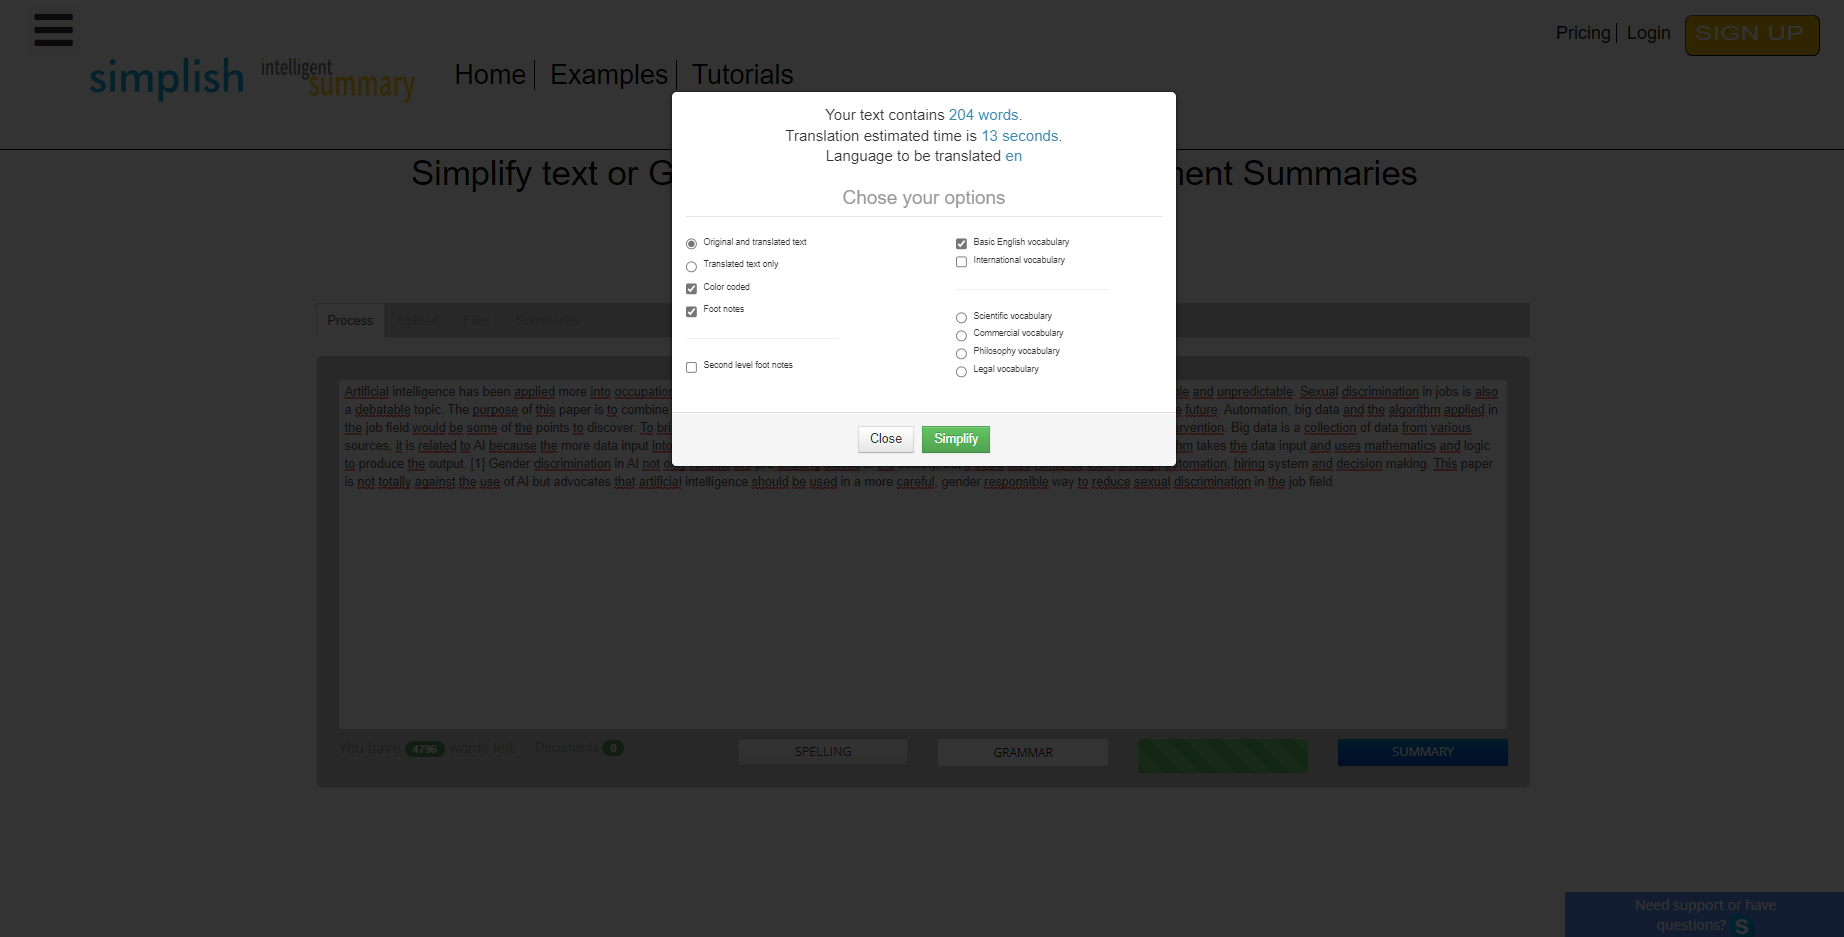
\includegraphics{img/simplish-input.png}
	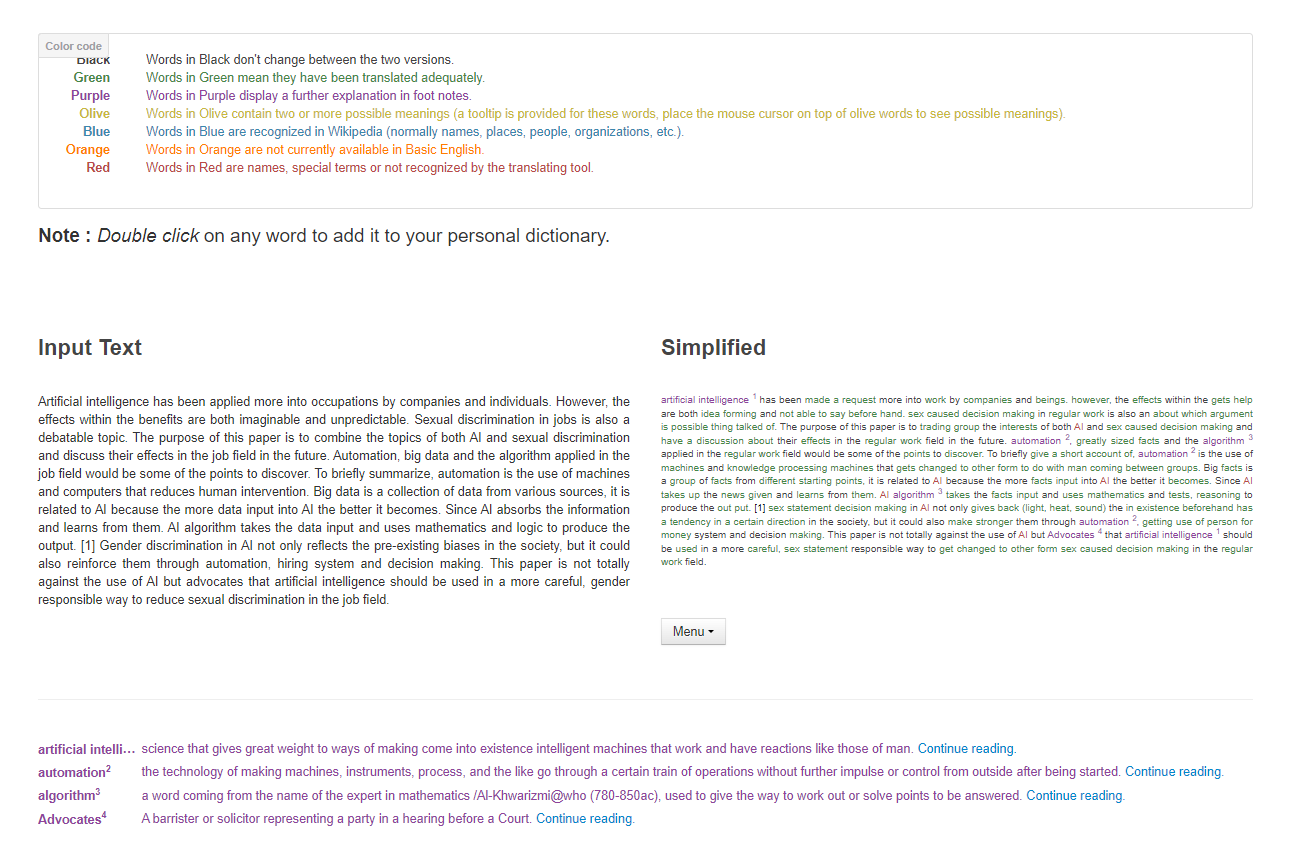
\includegraphics{img/simplish-output.png}
\end{figure}

\subsubsection{Syntactische vereenvoudiging}

\subsubsection{Samenvatten}

De experimenten met teksten wijzen uit dat GPT en Bing AI de nadruk legt op het behouden van bronreferenties. Wanneer expliciet gevraagd aan de Bing chatbot, geeft het model bronnen terug die buiten het oorspronkelijke artikel te vinden zijn.

\subsection{Conclusie}

\chapter{Prototype voor tekstvereenvoudiging}

\section{Voorbereiding}

\subsubsection{Python-notebooks}

De werking van tekstvereenvoudiging via Python-code wordt optimaal weergegeven in Python notebooks. Het gebruik van API's vormt geen hindernis en voorziet een snelle weergave zonder dat code uitgevoerd moet worden. 

\subsubsection{Keuze back-end en front-end}

Het prototype maakt gebruik van een Flask en het Jinja-framework. Aanvullend maakt het prototype gebruik van de nodige HTML- en CSS bestanden om de nodige visuele ondersteuning te kunnen aanbieden aan zowel lectoren als scholieren met dyslexie in de derde graad van het middelbaar onderwijs. Het aanspreken van de back-end vanuit de HTML-pagina's gebeurt met JavaScript-calls.

\subsubsection{Docker-omgeving}

Voor een optimale opzet als ontwikkelaar wordt er gebruik gemaakt van Docker. Een bat-scriptbestand maakt de opstart van deze lokale webapplicatie intuïtiever dan de opstart via een terminal. Daarnaast worden de benodigde Python-bibliotheken en taalmodellen alvorens opgehaald.

\subsubsection{PDF text mining}

De meest gebruikte vorm van tekstbestanden is in de vorm van PDF-bestanden. Methoden om deze bestanden uit te lezen en om te zetten naar tekstdata bestaan reeds in de vorm van Python-bibliotheken. De keuze van de bibliotheek speelt wel een rol. Sommige Python-bibliotheken bieden meer analyse- en verwerkingsfuncties aan. PDF Miner biedt extra functies aan om de metadata van een PDF-bestand op te halen of om classificatie op basis van lettertypes of pagina's per titel op te halen. Deze functies bevatten een intuïtieve naamgeving en besparen ontwikkelaars de overbodige werklast om extra logica te schrijven.

\subsubsection{Data pre-processing}

% todo stopword removal voor keyword extraction

\subsection{Extraherende samenvatting}

\subsubsection{BERT Extractive Summarization}

Indien niet aangegeven, wordt het aantal zinnen bepaald door het BERT-model.

\subsubsection{Vertaling}

BERT houdt geen rekening met vertaling. Het model staat enkel paraat om zinnen te markeren en de belangrijkste zinnen terug te geven. Voor de vertaling wordt de Google Translate Python-package gebruikt. Deze is minder accuraat vergeleken met DeepL, maar biedt een gratis beschikbaar en aanvaardbaar alternatief aan. Factoren zoals topic diversity en semantische redundantie moeten overwogen worden bij het kiezen van een taalmodel voor extraherend samenvatten.

\begin{lstlisting}[language=Python]
def extractive_summarization(full_text):

try:    
    from summarizer import Summarizer
    model = Summarizer()

    """determining optimal number of sentences based on MMR"""
    res = model.calculate_optimal_k(
        full_text, 
        k_max=10
    )

    """extracting key sentences"""
    result = model(
        body=full_text,
        max_length=700,
        min_length=100,
        num_sentences=res,
        return_as_list=True
    )

    new = []
    try:
        for i in result:
            if detect(i) != LANG:
                new.append(translate_sentence(i))
            else:
                new.append(i)
        return ' '.join(new)
    except Exception as e:
        return f'Problemen met Google Translate {e}'

except Exception as e:
    return f'Problemen met BERT {e}'
\end{lstlisting}

\subsection{Integreren naar Flask}

Flask biedt een snelle en toegankelijke opzet aan voor Python-ontwikkelaars. De combinatie van een robuuste front-end en back-end maakt dit binnen de schaal van een prototype ideaal.

\begin{lstlisting}

@app.route('/', methods=['GET'])
def home():
	return render_template('index.html')

if __name__ == "__main__":
	app.run()
\end{lstlisting}

% \subsection{title}

